\newpage
%%%%%%%%%%%%%%%%%%%%%%%%%%%%%%%%%%%%
%%%%%%%%        PCB         %%%%%%%%
%%%%%%%%%%%%%%%%%%%%%%%%%%%%%%%%%%%%

\section{Printed Circuit Board}\label{03Sec:PCB}



    


\subsection{PCB Design}\label{03Sub:PCBDesign}


\subsection{PCB Specifications}\label{03Sub:PCBSpecifications}

In the realm of electronic product development, PCB design plays a crucial role in ensuring the optimal 
functionality and performance of microcontroller-based systems. This section will highlight some of the key 
points covered in the microcontroller's hardware design guidelines \cite{ESP8266HGL}, along with best practices 
for PCB design. These guidelines provide valuable insights into the recommended approaches for designing the hardware 
layout, addressing critical aspects such as power supply, signal integrity, component placement, and grounding. 
By adhering to these guidelines and following established best practices, designers can achieve robust and reliable 
PCB designs that maximize the microcontroller's potential and minimize potential issues during manufacturing and 
operation.


\subsubsection{ESP8266EX Power Supply Design}\label{02SubSub:PowerSupplyDesign}


Prior to the power traces reaching the analog power-supply pins (Pin1, 3, 4, 28, 29), the inclusion of a 10 $\mu$F capacitor, working 
in conjunction with a 0.1 $\mu$F capacitor, becomes necessary. Additionally, an arrangement of a C circuit and an L circuit is advised 
for the power supplies of Pin3 and Pin4.The C-L-C circuit should be positioned as proximate as possible to the analog power-supply pin \cite{ESP8266HGL}. 
For more information about these components, refer to Figure \ref{02fig:analogAndDigitalSupplies1}.
It is crucial to acknowledge that the power supply pathway can be susceptible to damage as a consequence of abrupt current surges 
during the transmission of analog signals by ESP8266EX. Consequently, it is imperative to incorporate an additional 10$\mu$F capacitor, 
packaged in either 0603 or 0805 dimensions, to complement the existing 0.1$\mu$F capacitor \cite{ESP8266HGL}.

\subsubsection{Layers Design}\label{02SubSub:LayersDesign}

On \cite{ESP8266HGL} there are two suggested models regarding the number and dispositions of layers on a PCB
that uses ESP8266EX (and by extension, an 2.4GHz RF antenna). The model with four layers was chosen. Here are 
the specifications: 


\begin{itemize}
    \item The initial layer corresponds to the uppermost part and is designated as the TOP layer, utilized for 
    signal lines and component placement.
    \item The subsequent layer represents the GND layer, dedicated solely to establishing a comprehensive ground plane without 
    the inclusion of signal lines.
    \item The following layer constitutes the POWER layer, exclusively reserved for the positioning of power lines. In certain 
    unavoidable situations, it is admissible to incorporate some signal lines within this layer.
    \item Lastly, the final layer denotes the BOTTOM layer, exclusively allocated for signal line placement. It is discouraged 
    to mount components on this particular layer.
\end{itemize}

Also, the power tracks should have a minimum size of 15 mils. The value used was 20 mils.

\subsubsection{Reset Track Design}\label{02SubSub:ResetTrackDesign}

The EXT\_RSTB (Pin32) possesses an internal pullup resistor and operates on an active low mechanism. To mitigate the possibility
of external disturbances causing unwarranted resets, it is advised to maintain a concise PCB trace for EXT\_RSTB and 
incorporate an RC circuit at this pin \cite{ESP8266HGL} (see section \ref{02SubSub:RCDelayResetCircuitry}).



\subsubsection{XTAL - Crystal Oscillator Design}

To ensure proper functioning of the crystal oscillator, it is recommended to position it as close as possible to 
the XTAL pins, while considering the length of the traces. However, it is crucial to maintain an appropriate distance 
between the crystal and the chip to avoid any interference. The recommended distance from the MCU is 0.8 mm. 
This distance helps prevent any potential disruption caused by the crystal's  proximity to the chip. Additionally, it 
is important to note that there should be no vias present on the input and output traces. This means that the traces 
should not cross layers, ensuring a clean and uninterrupted signal path for the crystal oscillator. 
This design consideration helps maintain the integrity of the crystal oscillator's signals and enhances the overall 
performance of the circuit.

\subsubsection{RF Antenna}\label{03Sub:RFAntenna}

The RF impedance characteristic is 50$\Omega$, which indicates the desired impedance for optimal signal transmission. 
It is crucial to have a complete ground plane to ensure proper grounding and minimize interference. The RF trace should be kept as 
short as possible, and it is recommended to have dense ground via stitching surrounding it for isolation purposes. The width of RF 
lines should be minimized, and additional dense vias should be placed around them. A $\pi$-type matching circuitry (see the PCB
file .kicad\_pcb on the ``KiCad Projeto Tractian'' folder).
should be allocated 
on the RF trace and positioned in close proximity to the RF Pin2. It is important to avoid the use of vias for the RF trace. When routing 
the RF trace, a 135° angle is preferred, or circular arcs can be utilized for trace bends. Furthermore, the RF antenna should be placed at 
a distance from high-frequency transmitting devices, such as crystal oscillators, DDR, and specific high-frequency clocks (for example,
SPI Clocks). Additionally, it is essential to keep USB ports, USB-to-UART signal chips, and UART signal lines (including traces, vias, 
test points, headers, etc.) as far away from the antenna as possible. More specific iformations can be seen on \cite{ESP8266HGL}.
For the circuitry previous to the antenna, see the Figure \ref{02fig:RFAntennaCircuitry}. For the its PCB design, the
Texas SWRA117D 2.4GHz - Left \cite{TexasRFAntenna} was used. \\ 

For the  50$\Omega$ impedance on track design, the following values were used (Figure \ref{02fig:50ohmImpedanceDesignA}). The calculation was done using the 
\textbf{AppCad} \textit{software} \cite{AppCad}. Notice that the inputed values are in mils.


\begin{figure}[H]
    \centering
    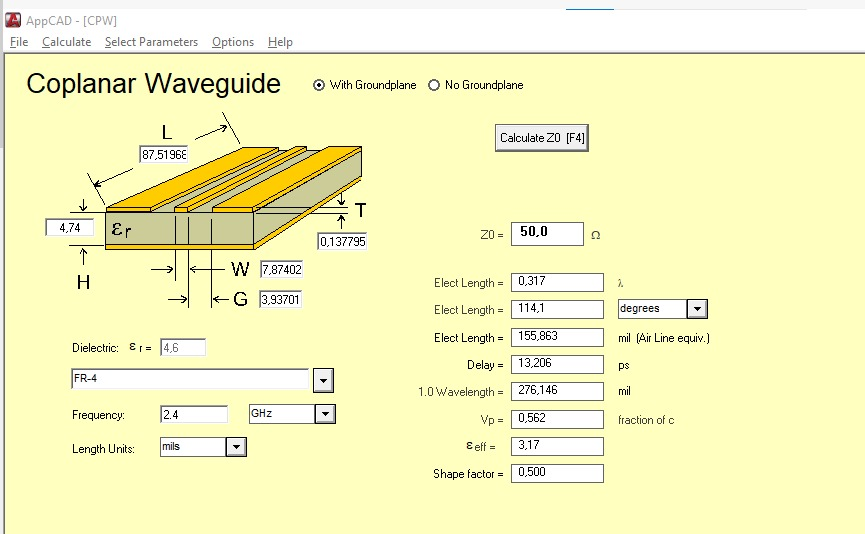
\includegraphics[scale = 0.6]{imagens/50ohmImpedanceDesignA.png}
    \caption{\textbf{Calculation of the 50$\Omega$ impedance - Coplanar Waveguide}.}
    \label{02fig:50ohmImpedanceDesignA}
\end{figure}










%%%%%%%%%%%     FIM      %%%%%%%%%%%  
%%%%%%%%        PCB         %%%%%%%%
%%%%%%%%%%%%%%%%%%%%%%%%%%%%%%%%%%%%